
\begin{frame}
\frametitle{3. ~ Conformal maps}

A \emph{\bfseries conformal map} between two regions of the plane is a transformation that preserves shapes infinitesimally.
More precisely: it preserves angles.

\bigskip
\pause

\begin{center}
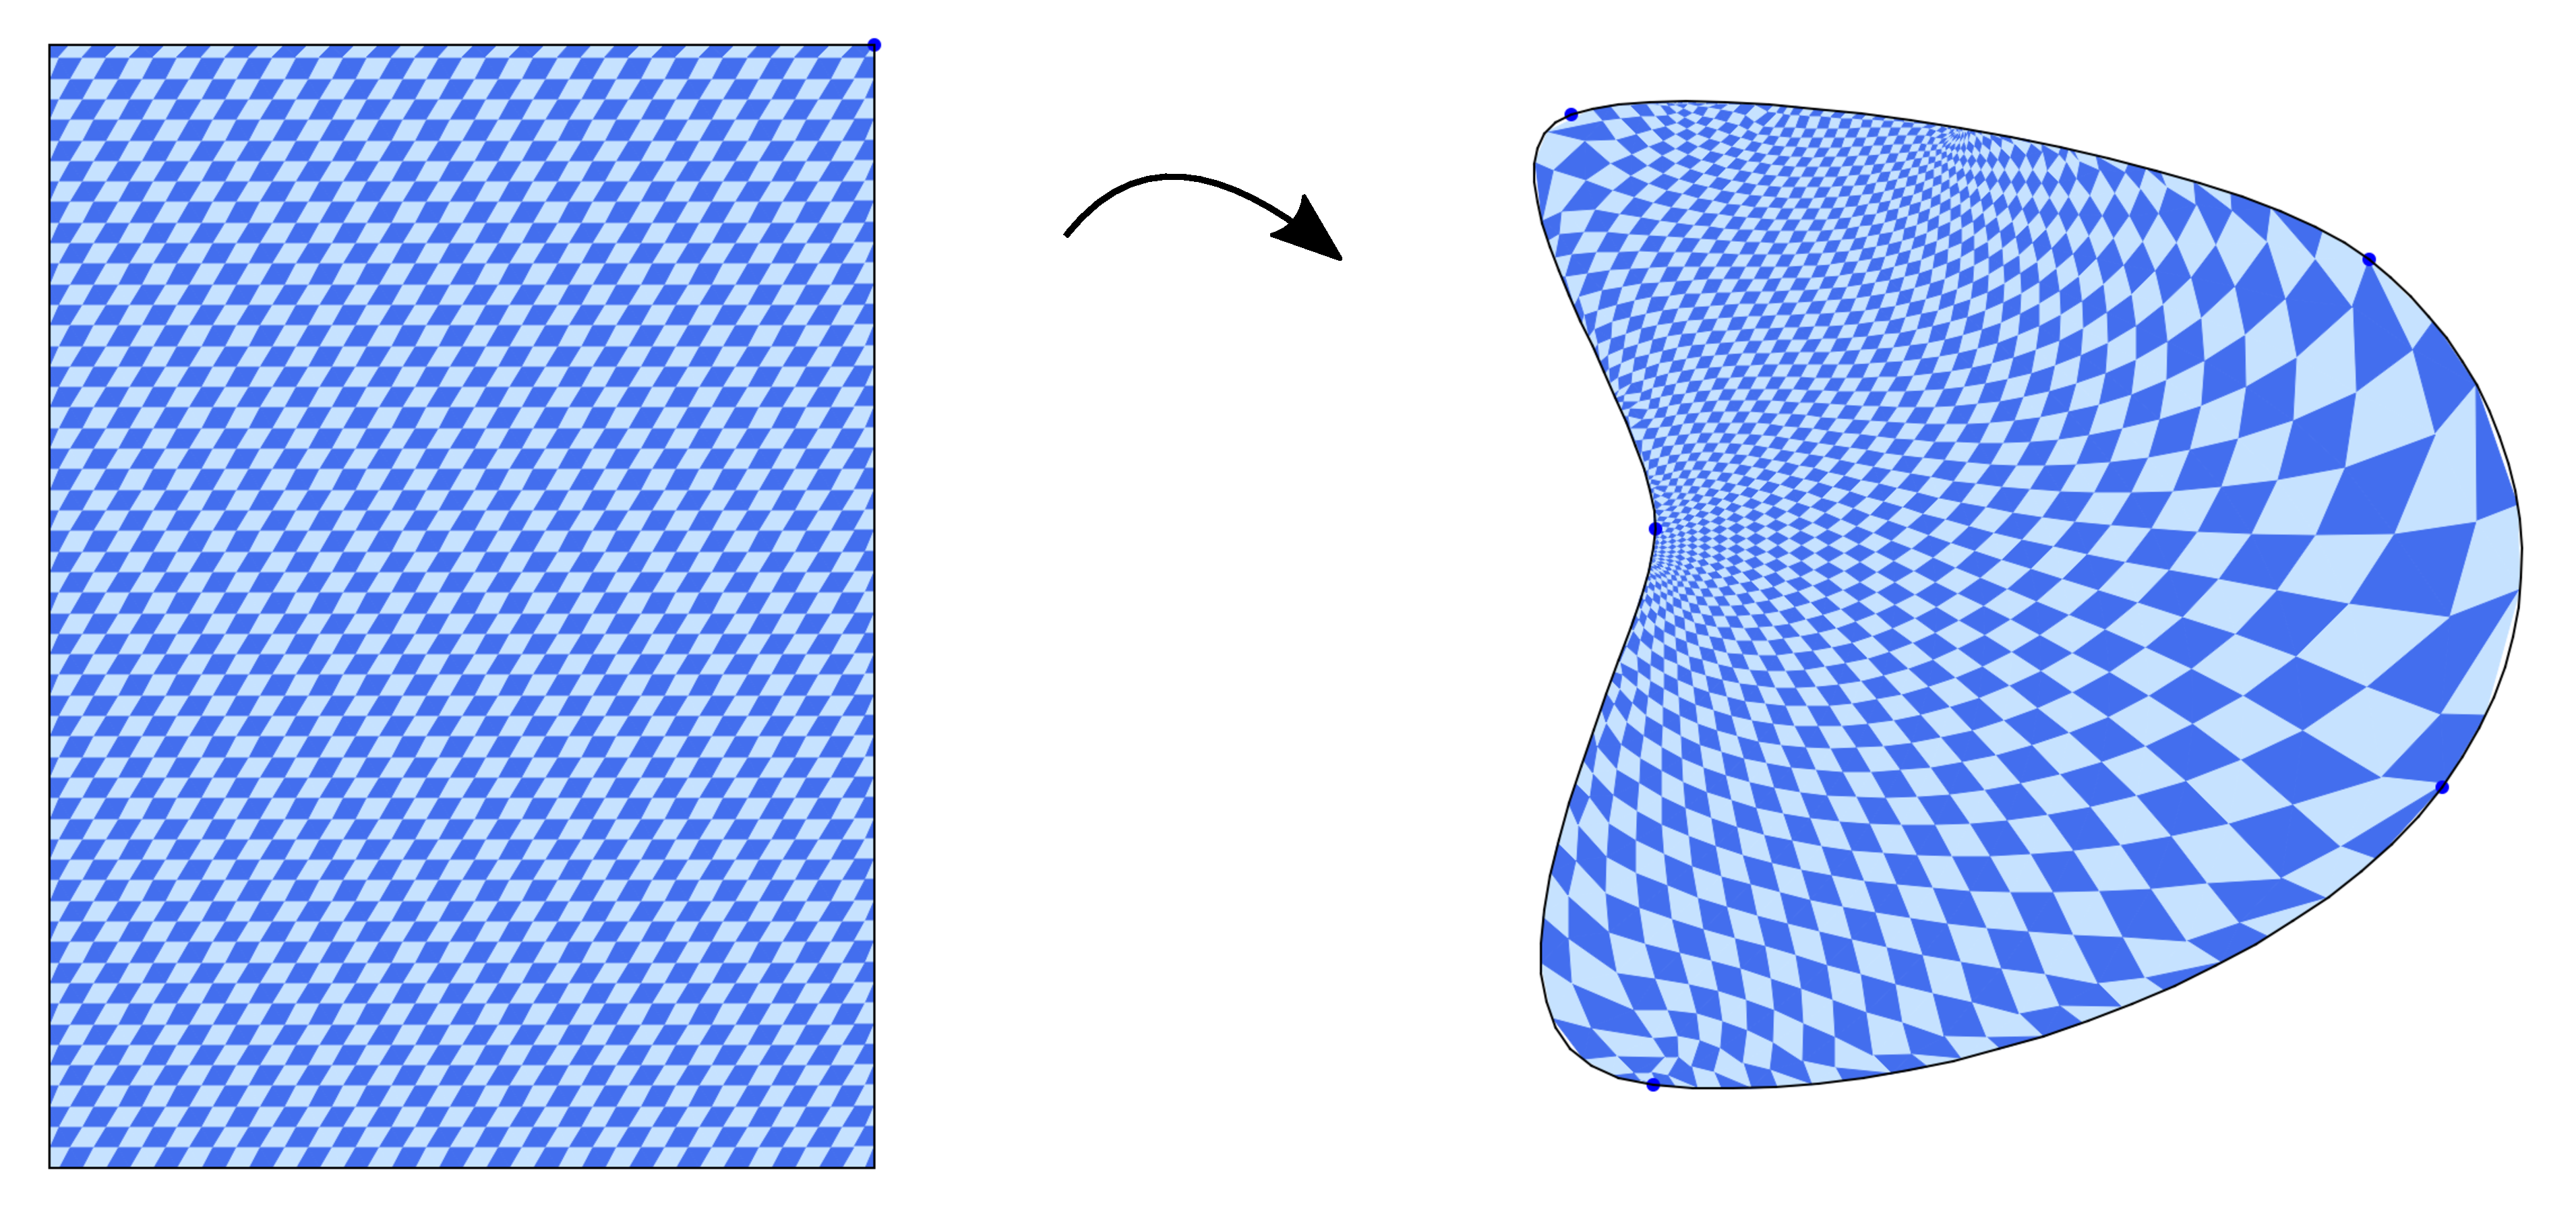
\includegraphics[width=\textwidth]{images/Conf1.pdf}
\end{center}

\end{frame}




\begin{frame}
\frametitle{3. ~ Conformal maps}

Conformal maps are intensely studied by mathematicians and have many important real-world applications.

\bigskip \pause

\begin{center}
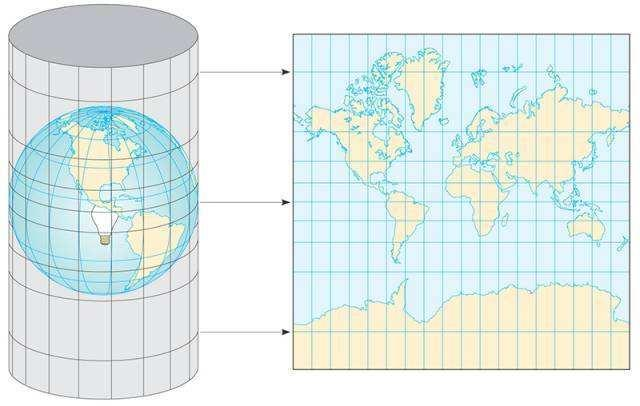
\includegraphics[height=110pt]{images/mercator3.jpg} \hspace{30pt} \pause
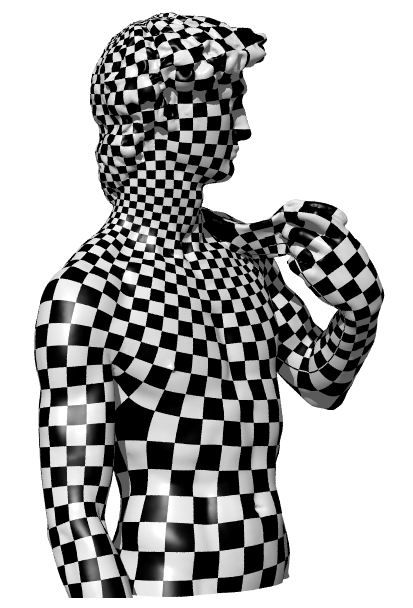
\includegraphics[height=130pt]{images/david.png}
\end{center}

\end{frame}



\begin{frame}
\frametitle{3. ~ Conformal maps}

\begin{theorem}[Riemann conformal mapping theorem]
Given any two simply-connected (no holes) regions $R_1$ and $R_2$ in the plane,
there exists a unique conformal map $f \colon R_1 \to R_2$.
\end{theorem}

\bigskip

\begin{center}
% {\includegraphics<1>[width=\textwidth]{images/Riemann1.png}}
{\includegraphics<2>[width=\textwidth]{images/Riemann1.png}}
{\includegraphics<3>[width=\textwidth]{images/Riemann2.png}}
\end{center}
\end{frame}






\begin{frame}
\frametitle{3. ~ Conformal maps}

How to compute conformal maps? \pause

\smallskip
$\longrightarrow$ \emph{Discrete conformal structures.}

\bigskip \pause
\textbf{Idea} (Thurston): Circle packings provide discrete conformal structures.


\end{frame}
